% !TEX root = ./report.tex

\clearpage
\section{The Inliner}
\label{sec:scheme}

The following heuristic is executed by the inliner of this project when given an
RVSDG as input:

\begin{enumerate}
	\item For all recursive environments ($\phi$-regions):

	\begin{enumerate}
		\item Use the approach described in
Section~\ref{sub:scheme:inlining_recur_apply_nodes} to fill a list \textit{loop
breakers}. These $\lambda$-nodes are \textit{not} to be inlined.
		\label{MakeLoopBreakerListItem}
	\end{enumerate}

	\item Scan through the RVSDG, finding all \applyNode s. Exclude all function
calls to loop breakers, calls invoking functions that are not-statically known,
or external functions.
	\label{ScanForApplyNodesItem}

	\item Make a list of the \applyNode s found in
Step~\ref{ScanForApplyNodesItem}, and order the list of according to the
heuristics discussed in Section~\ref{sub:scheme:ordering_apply_nodes}.
The order of \applyNode s inlined can affect the amount of \applyNode s inlined,
even when each \applyNode~is evaluated with the same heuristic.
	\label{OrderApplyNodesFoundItem}

	\item Look at each \applyNode~in turn from the list made in
Step~\ref{OrderApplyNodesFoundItem} and decide whether or not to inline it
according to the heuristic discussed in
Section~\ref{sub:scheme:inlining_apply_nodes}:
	\label{LookAtNextCallSiteItem}

	\begin{enumerate}
		\item If the \applyNode~is inlined, add any newly copied (inlined)
\applyNode s, following the same criteria as used in
Step~\ref{ScanForApplyNodesItem}, to the list of \applyNode s. Continue with
Step~\ref{OrderApplyNodesFoundItem}.

		\item If the \applyNode~is not inlined, continue with
Step~\ref{LookAtNextCallSiteItem}, evaluating the next \applyNode .
		\label{InlineCallSiteItem}
	\end{enumerate}

	\item When the inliner reaches the end of the list, no more \applyNode s
have been inlined, and the inliner is finished.
\end{enumerate}

\subsection{Deciding which recursive functions to inline}
\label{sub:scheme:inlining_recur_apply_nodes}

The inliner visits all \applyNode s and the functions they invoke functions,
with the same heuristic, described in
Section~\ref{sub:scheme:inlining_apply_nodes} regardless of whether the
functions invoked are recursive or not. However, the inliner of this project
only considers inlining \textit{some} of the \applyNode s invoking recursive
functions, to ensure termination of the compiler.

The \applyNode s not considered for inlining are the ones invoking \textit{loop
breakers}. Loop breakers are function-nodes found in $\phi$-regions which break
the Strongly Connected Component cycles within the $\phi$-region's call
dependency graph.

Loop breakers are found by visiting each function in the recursive environment
of a $\phi$-region, and then checking what functions its \applyNode s call. If
one of the \applyNode~calls a function already visited, the already visited
function is marked as a loop breaker. Hence, all self-recursive functions are
marked as loop breakers, but if two functions call each other in a cycle, only
one of them may be added to the list of loop breakers.

\todo[inline]{Make a figure or three of $\phi$-regions, one with a self-recursive
lambda, one with some mutually recursive ones (the example from PVV w/Torje),
and perhaps also one based on GHC papers FGHPQ example.}

Hence, the inliner has a list of recursive functions which it knows \textit{not}
to inline, thus ensuring termination of the compilation. All other remaining
recursive functions may then be safely inlined with the same criteria as any
non-recursive functions.

\subsection{The order of call sites inlined}
\label{sub:scheme:ordering_apply_nodes}

The heuristic deciding on whether or not to inline a specific \applyNode~is
based on previous work of Keith D. Cooper et. al~\cite{AdaptvStratInlSubst} and
Waterman~\cite{AdaptvCompilAndInlingWaterman}. Their work utilizes
\textit{Inlining Conditions} (ICs), which evaluate properties of the function
invoked or the call-site(s) invoking function.

\info[inline]{Because of above paragraph, which I think belongs to
Section~\ref{sub:scheme:inlining_apply_nodes}, ask Nico if he insists that
Section~\ref{sub:scheme:ordering_apply_nodes} should come before
Section~\ref{sub:scheme:inlining_apply_nodes}. I feel that this makes little
sense since the one that is first now relies on the second...}

As such, when a successive series of functions call one another, our approach
only considers one function's properties or \applyNode (s)'s properties,
depending upon the ICs used in the inlining heuristic, at a time. Some ICs such
as \textit{Node Count} (NC) can affect the amount of inlined \applyNode s,
depending on the order the \applyNode s are visited in.

Given the criteria for whether an \applyNode~is inlined is that the function it
invokes needs to contain less than four nodes, all of the \applyNode s in
Figure~\ref{fig:inline_ordering_ex} can be inlined, or just two of them. The
order the \applyNode s are visited in is what makes the difference in the amount
inlined given the inlining condition \lstinline!NC < 4!.

When the inliner visits the \applyNode s in Figure~\ref{fig:inline_ordering_ex}
top down, $\lambda_1$ can be inlined into $\lambda_2$. The new $\lambda_{1-2}$
can be inlined into $\lambda_3$, resulting in all of them being inlined into a
single function $\lambda_{1-2-3}$. However, if the \applyNode s are visited by
the inliner in a bottom up order instead, then $\lambda_3$ can be inlined into
$\lambda_2$, but $\lambda_{2-3}$'s NC exceeds 3, and cannot be inlined into
$\lambda_1$.

\begin{figure}[H]
	\centering
	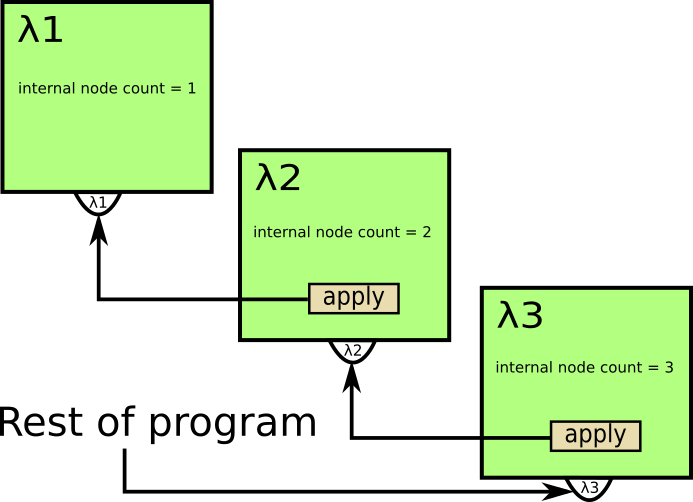
\includegraphics[width=0.75\textwidth]{figures/inline_ordering_ex}
	\caption{A minimal example of an RVSDG subgraph, depicting a function call
order in a program.}
	\label{fig:inline_ordering_ex}
\end{figure}

Both the top down and bottom up examples inlining $\lambda_1$, $\lambda_2$, and
$\lambda_3$, suppose that no other optimizations are applied on the inlined
code, meaning that no node which has gotten an \applyNode~inlined, will have
less nodes than the sum of its original NC plus the NC of the function inlined.

Because of this, our inliner is able to traverse the \applyNode s of an RVSDG in
a top down order, or a bottom up order.
Section~\ref{further_work:call_site_visit_order} discusses ideas for potential
work for future research on the impact of inlining call sites order.

\subsection{Inlining a call site}
\label{sub:scheme:inlining_apply_nodes}

Our approach was chosen because it permits effective testing for an apt
heuristic when deciding on whether or not to inline a call site.

As mentioned, the inliner uses several different ICs: NC, \textit{Static Call
Count} (SCC), and \textit{Loop Nesting Depth} (LND) being among these. SCC is
the total amount of \applyNode s for the function invoked, and LND is how many
nested loops the \applyNode~is located within.

These ICs and others described in Section~\ref{sub:meth:inlining_conditions},
allow us to write and re-write the inlining heuristic effectively, by letting us
write them using \textit{Conjunctive Normal Form} (CNF). Thus, the CNFs written
for our inliner heuristic are written in the following fashion:
\lstinline"NC < X || SCC < Y || (SCC < Z && LND > W)".

This permits us to efficiently search the parameter space for optimal parameters
for the inlining heuristics.

\todo[inline]{Describe the algorithm and inliner conditions we land for
evaluating a call site on after testing.}
